\documentclass[11pt,a4paper]{article}
\usepackage{graphicx}
\usepackage{amssymb, amsmath}
\usepackage{url}
\usepackage{polski}
\usepackage{subfigure}
\usepackage[utf8]{inputenc} 

\title{Współczesne techniki heurystyczne\\ Sprawozdanie nr 1.\\ \large Zastosowanie algorytmu rozmytego do sterowania prędkością samochodu}
\author{Piotr Jastrzębski\\ Marcin Nazimek}
\date{}
\begin{document}
\maketitle

\section{Szczegółowy opis zadania}\label{opis}
Rozważmy poruszający się samochód. W celu stworzenia modelu ruchu bierzemy pod uwagę dwie zmienne wejściowe: PRĘDKOŚĆ i ODLEGŁOŚĆ od jadącego z przodu samochodu oraz jedna zmienna określająca zmianę tego ruchu PRZYSPIESZENIE. Sterowanie odbywać będzie się poprzez zmianę prędkości. Przykładowe możliwe stany to: przyspieszenie, utrzymanie prędkości i hamowanie (ale można przyjąć więcej stanów, np. odległość jest bardzo mała, itp.).

Dla rozpatrywanego przypadku, baza reguł ma postać:
\begin{itemize}
\item IF odległość jest mała AND prędkość jest mała THEN utrzymaj prędkość.
\item IF odległość jest mała AND prędkość jest duża THEN zredukuj prędkość.
\item IF odległość jest duża AND prędkość jest mała THEN zwiekszaj prędkość.
\item IF odległość jest duża AND prędkość jest duża THEN utrzymaj prędkość.
\end{itemize}
Zmienne ODLEGŁOŚĆ, PRĘKDKOŚĆ i PRZYSPIESZENIE to zmienne lingwistyczne, które mogą przyjmować rozmyte wartości: krótki, długi, mała, duża, utrzymaj, zredukuj i zwiększaj. Projektant ma teraz za zadanie dobrać tak parametry zbiorów rozmytych i obszarów rozważań by odpowiadały one rzeczywistości w jak najlepszym stopniu.

\section{Założenia projektu}\label{zalozenia}
Projekt ma symulować i prezentować wykorzystanie algorytmu logiki rozmytej do sterowania prędkością samochodu w~możliwie największym stopniu odwzorowując rzeczywistość.

W przygotowanym środowisku na potrzeby prezentacji wykorzystane zostaną dwa uproszczone modele reprezentujące samochody -- pierwszy, dalej oznaczany jako $A$, będący samochodem, dla którego przygotowane zostanie sterowanie, oraz samochód $B$, który w sposób niedeterministyczny, ale zgodny z przepisami i realnymi wartościami przyspieszeń, będzie poruszał się przed $A$. Każdy z nich w~danej chwili czasu opisany będzie wartością przyspieszenia i~prędkości.

\subsection{Ograniczenia}
Na potrzeby projektu przyjęto następujące ograniczenia:
\begin{itemize}
\item \textbf{Prędkość} - przyjmuje wartości z zakresu $0\div140km/h$ \footnote{Założono, że ruch odbywa się na autostradzie w Polsce.}.
\item \textbf{Przyspieszenie} - jest zmienne w czasie. Kwestią do rozstrzygnięcia pozostaje, czy będzie ono takie samo czy przyjmie różne wartości dla opóźnienia i przyspieszenia. Na bazie zgromadzonych informacji odpowiednie wydaje się przyjęcie wartości przyspieszenia z zakresu $\langle-9\frac{m}{s^2};4\frac{m}{s^2}\rangle$\footnote{Wartości prawdziwe dla suchej nawierzchni.}.
\item \textbf{Odległość} - wyrażona w kilometrach dowolną nieujemną liczbą dziesiętną.
\end{itemize}

\subsection{Stan początkowy}
Przed rozpoczęciem symulacji stan układu (wartości poszczególnych parametrów) mogą być modyfikowane. Ustalane mogą być zarówno prędkość początkowa samochodu $A$ oraz $B$ jak i odległość między nimi. Celem symulacji jest tak sterować parametrami samochodu $A$, aby jechał on możliwie jak najbliżej poprzedzającego samochodu nie powodując kolizji (najechania).

\subsection{Implementacja}
W celu prezentacji działania algorytmu planowane jest wykorzystanie funkcjonalności zawartych w programie \emph{Matlab R2011a} wraz z rozszerzeniem \emph{Fuzzy Logic Toolbox}. Moduł ten zapewnia funkcje, narzędzia graficzne i elementy \emph{Simulink} dla systemów bazujących na logice rozmytej.

Wstępnie planuje się wykorzystanie jednej z dwóch koncepcji prezentacji:
\begin{itemize}
	\item moduł \emph{Simulink}, który za pomocą kontrolera \emph{Fuzzy Logic Controller} oraz połączeń i sprzężeń zwrotnych będzie realizował zależności zmiennych między $A$ oraz $B$. Do wyświetlania danych, m.in. wartości prędkości, odległości i przyspieszenia wykorzystane zostaną elementy typu \emph{Display} oraz {Scope}. Pierwsze próby, przedstawione na rysunku \ref{img:simulink1}, sprawiły jednak spore problemy ze względu na brak możliwości wymuszenia taktu symulacji na predefiniowaną wartość np. jedną sekundę.
	\item wykresu lub prostej animacji, która obrazować ma poprzez symbole zachowanie samochodów.
\end{itemize}

\begin{figure}
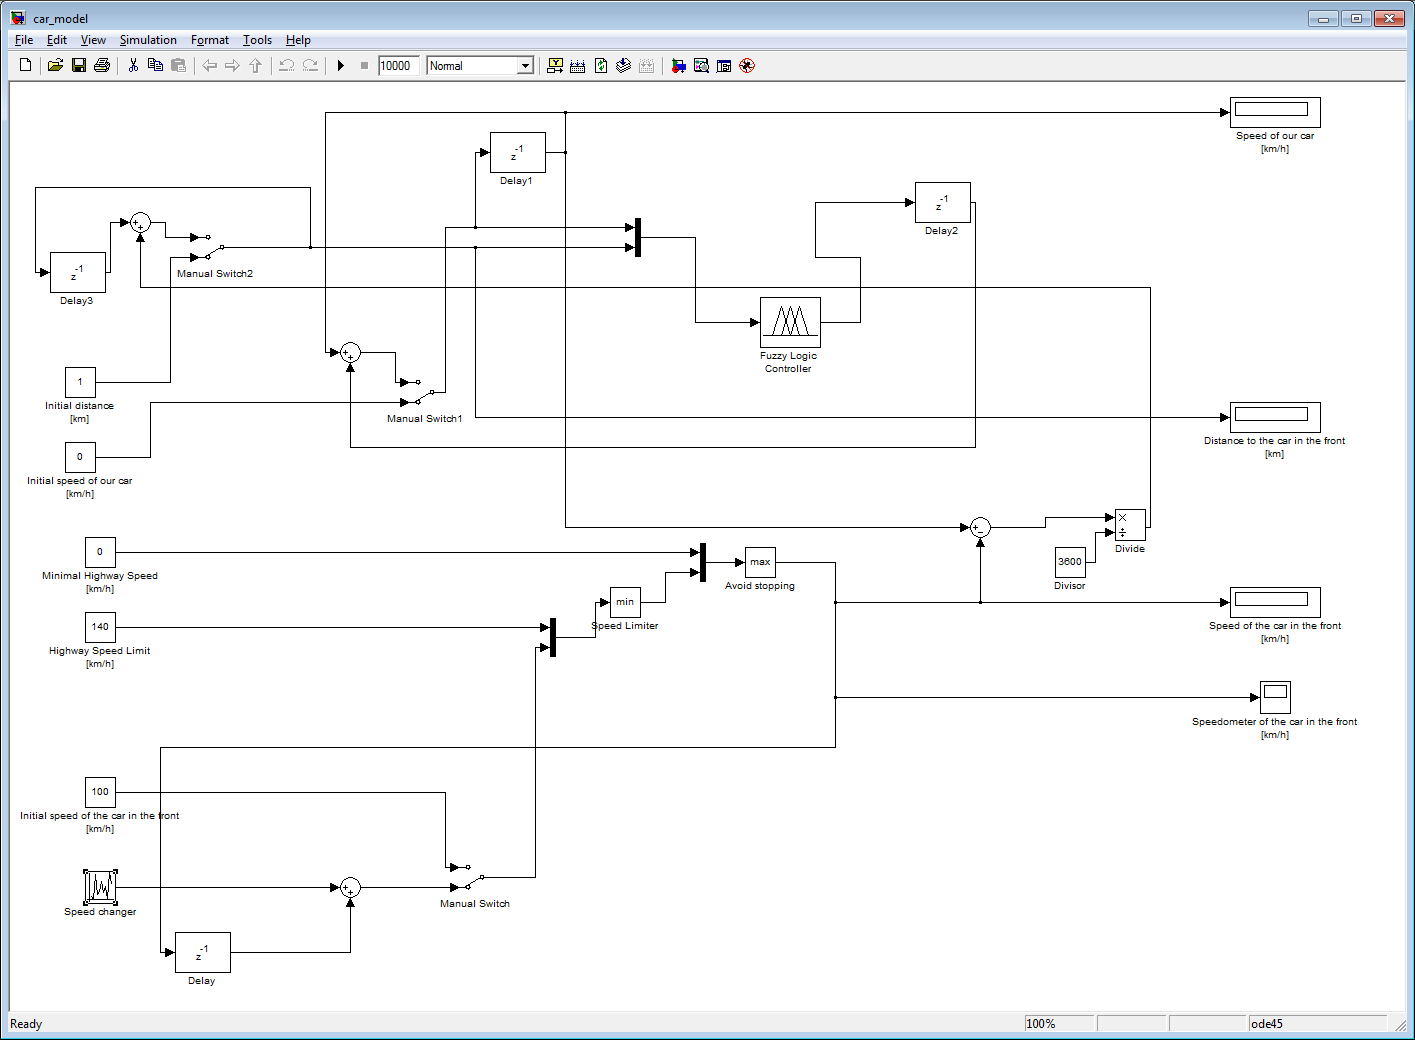
\includegraphics[width=\textwidth]{simulink1.png}
\caption{Układ wykonany w Simulink} 
\label{img:simulink1}
\end{figure}

\begin{thebibliography}{9}
	\bibitem{manual}
	\emph{Fuzzy Logic Toolbox User’s Guide}\\
	\url{http://www.mathworks.com/help/pdf_doc/fuzzy/fuzzy.pdf}

	\bibitem{engApp}
	Ross T., \emph{Fuzzy Logic with Engineering Applications}

	\bibitem{opis}
	Rykaczewski K., \emph{Systemy rozmyte i ich zastosowania}\\
	\url{http://math.uni.lodz.pl/~fulmanp/zajecia/ssn/materialy/duszek.pdf}
\end{thebibliography}

\end{document}
